%>>>>>>>>>>>>>>>>>>>>>>>>>> ПЕРЕМЕННЫЕ >>>>>>>>>>>>>>>>>>>>>>>>>>>>>>>>>>>
%>>>>> Информация о кафедре
%\newcommand{\year}{2021 г.}  % Год устанавливается автоматически
\newcommand{\city}{Санкт-Петербург}  %  Футер, нижний колонтитул на титульном листе
\newcommand{\university}{Национальный исследовательский университет ИТМО}  % первая строка
\newcommand{\department}{Факультет программной инженерии и компьютерной техники}  % Вторая строка
\newcommand{\major}{Направление программная инженерия}  % Треьтя строка
% Пусть будет. Проще закоментить лишнее.
\newcommand{\education}{Образовательная программа системное и прикладное программное обеспечение}  % четвертая строка
%\newcommand{\specialization}{}  % пятая строка

%<<<<< Информация о кафедре

%>>>>> Назание работы
\newcommand{\reporttype}{ОТЧЕТ ПО ЛАБОРАТОРНОЙ РАБОТЕ} % тип работы, (главный заголовок титульного листа)
\newcommand{\lab}{Лабораторная работа}          % вид работы
\newcommand{\labnumber}{№ 1}                    % порядковый номер работы
\newcommand{\subject}{Информатика}         % учебный предмет
\newcommand{\labtheme}{Принципы ООП}            % Тема лабораторной работы
\newcommand{\variant}{№ 4}                % номер варианта работы

\newcommand{\student}{Бых Даниил Максимович}    % определение ФИО студента
\newcommand{\studygroup}{P3109}                 % определение учебной группы
\newcommand{\teacher}{% принимающий
    Малышева Т. А.% ФИО практика
}
%<<<<<<<<<<<<<<<<<<<<<<<<<< ПЕРЕМЕННЫЕ <<<<<<<<<<<<<<<<<<<<<<<<<<<<<<<<<<<


%>>>>>>>>>>>>>>>>>>>>>> ПРЕАМБУЛА >>>>>>>>>>>>>>>>>>>>>>>>>
\documentclass[14pt,final,oneside]{extreport}% класс документа, характеристики
%>>>>> Разметка документа
\usepackage[a4paper, mag=1000, left=3cm, right=1.5cm, top=2cm, bottom=2cm, headsep=0.7cm, footskip=1cm]{geometry} % По ГОСТу: left>=3cm, right=1cm, top=2cm, bottom=2cm,
\linespread{1} % межстройчный интервал по ГОСТу := 1.5
%<<<<< Разметка документа

\setlength{\parindent}{1.25cm}

%>>>>> babel c языковым пакетом НЕ должны быть первым импортируемым пакетом
\usepackage[utf8]{inputenc}
\usepackage[T1,T2A]{fontenc}
\usepackage[russian]{babel}
% \usepackage{lmodern}
%<<<<<

%\usepackage{cmap} %поиск в pdf

%>>>...>> прочие полезные пакеты
\usepackage{amsmath,amsthm,amssymb}
\usepackage{mathtext}
\usepackage{braket}
\usepackage{indentfirst}
\usepackage{graphicx}
\usepackage{float}
\usepackage{changepage}
\graphicspath{{assets}}
\DeclareGraphicsExtensions{.pdf,.png,.jpg}
%\usepackage{bookmark}

\usepackage[dvipsnames]{xcolor}
\usepackage{hyperref}  % Использование ссылок
\hypersetup{%  % Настройка разметки ссылок
    colorlinks=true,
    linkcolor=blue,
    filecolor=magenta,
    urlcolor=magenta,
%pdftitle={Overleaf Example},
%pdfpagemode=FullScreen,
}

\usepackage{diagbox}
\usepackage[letterspace=150]{microtype} % Спэйсинг (межбуквенный интервал для саголовка) \lsstyle
% \usepackage{csvsimple} %импорт содержимого таблицы из csv

%>>> верстка в 2 колонки
\usepackage{multicol} % многоколоночная верстка
\setlength{\columnsep}{.15\textwidth} % определение ширины разделителя между колонками

\usepackage{tikz} % пакет для векторной графики, чтобы рисовать красивый разделитель колонок
% %> кастомный разделитель колонок
% \usetikzlibrary{arrows.meta,decorations.pathmorphing,backgrounds,positioning,fit,petri}
% \usepackage{multicolrule} % Для кастомизации разделителя колонок
% \SetMCRule{                     % кастомизация разделителя колонок multicolrule
%     width=2pt,
%     custom-line={               % Tikz код для кастомизации линии разделителя
%         \draw [                 % Рисовать
%             decorate,           % декорированную (требуются спец настройки пакетов tikz (см. импорт выше)
%             decoration={        % вид декорирования
%                 snake, % Тип - змейка (волнистая)
%                 amplitude=.5mm, % ширина волн
%                 pre length=0mm, % участок прямой линии от начала
%                 %segment length=0mm, % учасок волнистой линии
%                 post length=0mm % участок прямой линии от конца
%             },
%             line width=1pt,
%             step=10pt
%         ] 
%         (TOP) to (BOT); % сверху и до низа колонки
%     }, 
%     extend-top=-5pt, % Вылезти за верхнюю границу колонки 
%     extend-bot=-7pt % Вылезти за нижнюю границу колонки  
% }
%% < кастомный разделитель колонок
%%<<< верстка в 2 колонки

%>>>>> Использование листингов
\usepackage{listings}
\usepackage{caption}
\DeclareCaptionFont{white}{\color{white}}
\DeclareCaptionFormat{listing}{\colorbox{gray}{\parbox{\textwidth}{#1#2#3}}}

\captionsetup[lstlisting]{format=listing,labelfont=white,textfont=white} % Настройка вида описаний
\lstset{  % Настройки вида листинга
    inputencoding=utf8, extendedchars=\true, keepspaces = true, % поддержка кириллицы и пробелов в комментариях
    language={},            % выбор языка для подсветки (здесь это Pascal)
    basicstyle=\small\sffamily, % размер и начертание шрифта для подсветки кода
    numbers=left,               % где поставить нумерацию строк (слева\справа)
    numberstyle=\tiny,          % размер шрифта для номеров строк
    stepnumber=1,               % размер шага между двумя номерами строк
    numbersep=5pt,              % как далеко отстоят номера строк от подсвечиваемого кода
    backgroundcolor=\color{white}, % цвет фона подсветки - используем \usepackage{color}
    showspaces=false,           % показывать или нет пробелы специальными отступами
    showstringspaces=false,     % показывать илигнет пробелы в строках
    showtabs=false,             % показывать или нет табуляцию в строках
    frame=single,               % рисовать рамку вокруг кода
    tabsize=2,                  % размер табуляции по умолчанию равен 2 пробелам
    captionpos=t,               % позиция заголовка вверху [t] или внизу [b]
    breaklines=true,            % автоматически переносить строки (да\нет)
    breakatwhitespace=false,    % переносить строки только если есть пробел
    escapeinside={\%*}{*)}      % если нужно добавить комментарии в коде
}

\definecolor{codegreen}{rgb}{0,0.6,0}
\definecolor{codegray}{rgb}{0.5,0.5,0.5}
\definecolor{codepurple}{rgb}{0.58,0,0.82}
\definecolor{backcolour}{rgb}{0.95,0.95,0.92}

\lstdefinestyle{mystyle}{
backgroundcolor=\color{backcolour},
commentstyle=\color{codegreen},
keywordstyle=\color{magenta},
numberstyle=\tiny\color{codegray},
stringstyle=\color{codepurple},
basicstyle=\ttfamily\footnotesize,
breakatwhitespace=false,
breaklines=true,
captionpos=b,
keepspaces=true,
numbers=left,
numbersep=5pt,
showspaces=false,
showstringspaces=false,
showtabs=false,
tabsize=2
}
\lstset{style=mystyle}
%<<<<< Использование листингов


\sloppy % Решение проблем с переносами (с. 119 книга Львовского)
\emergencystretch=25pt


%>>>>>>>>>>>>>>>> ДОПОЛНИТЕЛЬНЫЕ КОМАНДЫ {Для соответствия ГОСТ} >>>>>>>>>>>>>>
%>>>>>> математические функции для удобства
\newcommand{\tx}{\text}
\newcommand{\eps}{\varepsilon}
\renewcommand{\phi}{\varphi}
\newcommand{\limit}{\displaystyle\lim}
\newcommand{\oo}{\infty}
\newcommand{\De}{\Delta}
\newcommand{\cd}{\cdot}
\newcommand{\df}{\partial}
\newcommand{\ndash}{\textendash}
\newcommand{\mdash}{\textemdash}

%>>>>> Аннотирование
\newcommand{\note}[2]{\overbrace{#1}^{#2}}% скобка сверху для комментария
% \overset{}{}% для указания символа над другим смиволом
% \underset{}{}% для указания символа под другим смиволом
%<<<<< Аннотирование

%>>>>>> Матрицы
\DeclareMathOperator{\rank}{rank}
\newcommand{\tvec}[1]{\mathbfit{#1}}% "text vector"
\newcommand{\mtx}[1]{\mathrm{#1}}
\newcommand{\transposed}[1]{{#1}^{\mathrm{T}}}
%>>>>>> Матрицы

%>>>>> Скобки
\newcommand{\lt}{\left}
\newcommand{\rt}{\right}
\newcommand{\la}{\langle}% '<'
\newcommand{\ra}{\rangle}% '>'
\newcommand{\avg}[1]{\langle{#1}\rangle}% '<X>'
%<<<<< Скобки

%>>>>> Дроби
\newcommand{\cf}[2]{\cfrac{#1}{#2}}
\newcommand{\fr}[2]{\frac{#1}{#2}}
%<<<<< Дроби


%>>>>> Стрелки
\newcommand{\Rarr}{\Rightarrow}% ⇒ следствие | лучше использовать \implies
\newcommand{\LRarr}{\Leftrightarrow}% равносильно | лучше  использовать \iff
\newcommand{\rarr}{\xrightarrow{}}% → стрелка вправо
\newcommand{\nwarr}{\nwarrow}% ↖ север-запад стрелка
\newcommand{\nearr}{\nearrow}% ↗ север-восток стрелка
\newcommand{\swarr}{\swarrow}% ↙ юг-запад стрелка
\newcommand{\searr}{\searrow}% ↘ юг-восток стрелка

\newcommand{\raises}{\nwarrow}% возрастает
\newcommand{\increases}{\nwarrow}% возрастает
\newcommand{\falls}{\swarrow}% убывает
\newcommand{\decreases}{\swarrow}% убывает

%{{{
\makeatletter
\newcommand{\impliesby}[2][]{\ext@arrow 0359\Leftrightarrowfill@{#1}{#2}}% следствие с надписью
\makeatother
%}}}

%{{{
\makeatletter
\newcommand{\iffby}[2][]{\ext@arrow 0359\Rightarrowfill@{#1}{#2}}% равносильность с надписью
\makeatother
%}}}
%<<<<< Стрелки

% Функции для удобного описания формул: https://tex.stackexchange.com/questions/95838/how-to-write-a-perfect-equation-parameters-description


%<<<<<< математические функции для удобства
%>>>>>> Стиль текста
\newcommand{\hex}[1]{\texttt{0{\footnotesize{x}}#1}}
\newcommand{\ttt}[1]{\texttt{#1}}
%<<<<<< Стиль текста

\newcommand\Chapter[3]{%
% Принимает 3 аргумента - название главы и дополнительный заголовок и множитель ширины загловка (можно ничего)
\refstepcounter{chapter}%
\chapter*{%
%\hfill % заполнение отступом пространства до заголовка
\begin{minipage}{#3\textwidth} % Можно изменить ширину министраницы (заголовка)
\flushleft % Выранивание заголовка по левому краю параграфа (заголовка)
%\flushright % Выранивание заголовка по правому краю параграфа (заголовка)
\begin{huge}%
% Отключена нумерация глав в тексте:
% \textbf{\chaptername\ \arabic{chapter}\\}
\textbf{#1}% Первый заголовок
\end{huge}%
\\% Перенос сторки
\begin{Huge}
#2% Второй заголовок
\end{Huge}
\end{minipage}
}%
% Отключена нумерация для chapter в toc (table of contents), т.е. Оглавлении (Содержании):
% \addcontentsline{toc}{chapter}{\arabic{chapter}. #1}
% Представление главы в содержании:
\addcontentsline{toc}{chapter}{#1. #2}%
}

\newcommand\Section[1]{
% Принимает 1 аргумент - название секции
\refstepcounter{section}
\section*{%
\raggedright
% Отключена дополнительная нумерация chapter в section в тексте документа:
% \arabic{chapter}.\arabic{section}. #1}
% Отключена любая нумарация section в тексте документа:
\arabic{section}. #1%
}

% Отключена дополнительная нумерация chapter в section в toc (table of contents) Оглавлении (Содержании):
% \addcontentsline{toc}{section}{\arabic{chapter}.\arabic{section}. #1}
\addcontentsline{toc}{section}{\arabic{section}. #1}
}


\newcommand\Subsection[1]{
% Принимает 1 аргумент - название подсекции
\refstepcounter{subsection}
\subsection*{%
\raggedright%
% Отключена дополнительная нумерация chapter в section в тексте документа (можно добавить отступ с помощью \hspace*{12pt}):
% \arabic{chapter}.\arabic{section}.\arabic{subsection}. #1}
\arabic{section}. \arabic{subsection}. #1
}
% Отключена дополнительная нумерация chapter в section в Оглавлении (Содержании):
%\addcontentsline{toc}{subsection}{\arabic{chapter}.\arabic{section}.\arabic{subsection}. #1}
\addcontentsline{toc}{subsection}{\arabic{subsection}. #1}
}


\newcommand\Figure[4]{
% Принимает 4 аргумента - название файла изображения, ее размер в тексте, описание, лэйбл (псевдоним в формате "fig:name")
%
\refstepcounter{figure}
\begin{figure}[H] %- \usepackage {float} %[h]
\begin{center}
\fbox{
\includegraphics[width=#2]{#1}
}
\end{center}
\begin{center}
Рис.~\arabic{figure}. #3.
\end{center}
%\caption{#3}
\label{fig:#4}
\end{figure}
}


\newcommand\Table[3]{
% Принимает 3 аргумента --- лэйбл name(#1) (псевдоним в формате "tab:name"), ее описание(#2), содержание таблицы(#3)
% ВАЖНО!: от этого способа страдает нумерация описаний, можно использовать создание таблиц через googlesheet
%
\renewcommand{\arraystretch}{1.2} % Установка высоты строки таблицы по умолчанию, увеличенное на 0.2 пункта
% \refstepcounter{table}% увеличение счетчика таблиц
\begin{table}[Htpb]% "right Here", "top", "new page", "bottom"
\label{tab:#1}% лэйбл таблицы, для ссылок
\resizebox{\columnwidth}{!}{% сжимает очень широкие таблицы, чтобы вместить на страницу
#3% Содержимое таблицы
}
%
\caption{#2}% Описание стандартными средствами для используемого окружения (table)
% \captionof{table}{#2}% Описание стандартными средствами
% \captionof*{figure}{\flushleft \textsc\textbf{Рис. 1.}}% Описание стандартными средствами, как рисунка
%
%%> кастомное описание
% \begin{flushleft}% Кастомное описание
%     % \textsf{%
%         \textbf{%
%             \\[2mm]
%             #2% Описание к картинке
%         }%
%         % \\[8mm]% Отступ
%     % }%
% \end{flushleft}
%%< кастомное описание
\end{table}
\renewcommand{\arraystretch}{1} % возврат установка высоты строки таблицы по умолчанию на 1
}


\newcommand\CustomFigure[4]{ % multicols не умеют в table и figure, поэтому приходится извращаться % вставка таблицы с меткой рисунка
% Принимает 4 аргумента - название файла изображения, ее размер в тексте, описание, лэйбл (псевдоним в формате "fig:name")
%
\refstepcounter{figure}
\begin{figure}[ht]% "here", "top"
\begin{center}
\includegraphics[width=#2]{#1}
\end{center}
%
%\caption{#3}
\captionof{figure}{#3}% описание стандартными средствами
% \begin{center}
\begin{flushleft} % Кастомное описание
\textbf{%
#3% Текст описания
}
\end{flushleft}
% \end{center}
%
\label{fig:#4}% Лэйбл, для ссылок
\end{figure}
}


\newcommand\CustomTableFigure[3]{% multicols не умеют в table и figure, поэтому приходится извращаться % вставка таблицы с меткой рисунка
%
% Принимает 3 аргумента --- лэйбл name(#1) (псевдоним в формате "tab:name"), ее описание(#2), содержание таблицы(#3)
%
\begin{center}
\refstepcounter{figure}
\label{tab:#1}% лэйбл таблицы, для ссылок
\resizebox{\columnwidth}{!}{% сжимает очень широкие таблицы, чтобы вместить на страницу
#3% Содержание таблицы
}
%
\captionof{figure}{#2}% Описание стандартными средствами
% \captionof*{figure}{\flushleft \textsc\textbf{Рис. 1.}}% Описание стандартными средствами
%
\begin{flushleft}% Кастомное описание
% \textsf{%
\textbf{%
\\[2mm]
#2% Описание к картинке
}%
% \\[8mm]% Отступ
% }%
\end{flushleft}
\end{center}
}


\newcommand{\InkscapeFigure}[4]{% Вставки иллюстраций из Inkscape (pdf+latex)
%
% Принимает 4 параметра: #1 название файла, #2 описание, #3 лейбл #4 размер
%
% \begin{minipage}{#4}
\begin{figure}[htbp]
\centering
\def\svgwidth{#4}
\import{./figures/}{#1.pdf_tex}
\caption{#2}
\label{fig:#3}
\end{figure}
% \end{minipage}
}


\newcommand\Equation[3]{% Кастомное оформление выражений
%
% Принимает 3 аргумента --- лэйбл name (#1) (псевдоним в формате "tab:name"), его описание(#2), содержание выражения (#3)
%
\textbf{#2}% описание
\begin{equation}
#3% содержимое выражений
\label{eq:#1}% лэйбл
\end{equation}
}

%<<<<<<<<<<<<<<<<<<<<<<<<<<<< ДОПОЛНИТЕЛЬНЫЕ КОМАНДЫ <<<<<<<<<<<<<<<<<<<<<<<<<<
%<<<<<<<<<<<<<<<<<<<<<< ПРЕАМБУЛА <<<<<<<<<<<<<<<<<<<<<<<<<


%%%%%%%%%%%%%%%%%%% СОДЕРЖИМОЕ ОТЧЕТА %%%%%%%%%%%%%%%%%%%%%
%>>>>>>>>>>>>>>> ''''''''''''''''''''''' >>>>>>>>>>>>>>>>>>
\begin{document}


%>>>>>>>>>>>>>>>> ОПРЕДЕЛЕНИЕ НАЗВАНИЙ >>>>>>>>>>>>>>>>>>>>
% Переоформление некоторых стандартных названий
%\renewcommand{\chaptername}{Лабораторная работа}
    \renewcommand{\chaptername}{\lab\ \labnumber} % переименование глав
    \renewcommand{\contentsname}{Содержание} % переименование оглавления
%<<<<<<<<<<<<<<<< ОПРЕДЕЛЕНИЕ НАЗВАНИЙ <<<<<<<<<<<<<<<<<<<<
% \setlength{\itemsep}{0pt} % установка расстояния между строчками в списках можно использовать локально внутри списка списке
% \setlength{\parskip}{0pt} % 
% \setlength{\parsep}{0pt}  % 

%>>>>>>>>>>>>>>>>> ТИТУЛЬНАЯ СТРАНИЦА >>>>>>>>>>>>>>>>>>>>>
    %>>>>>>>>>>>>>>>>>>> ТИТУЛЬНЫЙ ЛИСТ >>>>>>>>>>>>>>>>>>>>>>>
\begin{titlepage}

    % Название университета
    \begin{center}
        \textsc{%
            \university\\[5mm]
            \department\\[2mm]
            \major\\
            \education\\
%        \specialization\\
        }

        \vfill
        % Название работы
        \textbf{\reporttype\ \labnumber\\[3mm]
        курса <<\subject>> \\[6mm]
%    по теме: <<\labtheme>>\\[3mm]
        Вариант \variant\\[20mm]
        }
    \end{center}


    \vfill
    \hfill
% Информация об авторе работы и проверяющем
    \begin{minipage}{.5\textwidth}
        \begin{flushright}


            Выполнил студент:\\[2mm]
            \student\\[2mm]
            группа: \studygroup\\[5mm]

            Проверил:\\[2mm]
            \teacher

        \end{flushright}
    \end{minipage}

    \vfill

    % Нижний колонтитул первой страницы
    \begin{center}
        % 
\includegraphics[width=3cm]{itmo_logo.png}
        % \\
        \city, \the\year\,
    \end{center}

\end{titlepage}

%<<<<<<<<<<<<<<<<< ТИТУЛЬНАЯ СТРАНИЦА <<<<<<<<<<<<<<<<<<<<<


%>>>>>>>>>>>>>>>>>>>>> СОДЕРЖАНИЕ >>>>>>>>>>>>>>>>>>>>>>>>>
% Содержание
    \tableofcontents
%<<<<<<<<<<<<<<<<<<<<< СОДЕРЖАНИЕ <<<<<<<<<<<<<<<<<<<<<<<<<


%%%%%%%%%%%%%%%%%%%%%%% КОД РАБОТЫ %%%%%%%%%%%%%%%%%%%%%%%%
%>>>>>>>>>>>>>>>>>>>'''''''''''''''''>>>>>>>>>>>>>>>>>>>>>
    \newpage
    % \Chapter{\lab\ \labnumber}{}{}

    \Section{Задание}

    \noindent
%    \textbf{
%    % Заглавное описание....:
%        Заголовок
%    }
%
%    \textit{
%    % Описание задания...
%        Описание
%    }

    \begin{enumerate}
        \setlength{\itemsep}{0pt} % Сокращение межстрочных расстояний
        \setlength{\parskip}{0pt}
        \setlength{\parsep}{0pt}
        \item Перевести число А, заданное в системе счисления В, в систему
            счисления С. Числа А, В и С взять из представленных ниже
            таблиц. Вариант выбирается как сумма произведения 4-й и 5-й цифры номера ISU и 6-й цифры номера ISU. То есть если номер ISU = 125598, то это 5*9 + 8 = 45 + 8 = 53 - 40 = 13-й вариант. Если номер ISU = 467205, то это 2*0 + 5 = 7-й вариант;
        \item Обязательное задание (позволяет набрать до 85 процентов от
            максимального числа баллов БаРС за данную лабораторную). Всего
            нужно решить 13 примеров. Для примеров с 5-го по 7-й выполнить
            операцию перевода по сокращенному правилу (для систем с основанием
            2 в системы с основанием ${2^k}$). Для примеров с 4-го по 6-й и с 8-го по 9-
            й найти ответ с точностью до 5 знака после запятой. В примере 11 группа
            символов \{\^1\} означает -1 в симметричной системе счисления;
        \item Дополнительное задание №1 (позволяет набрать +15 процентов от
            максимального числа баллов БаРС за данную лабораторную). Написать
            программу на любом языке программирования, которая бы на вход
            получала число в системе счисления "С" из примера 11, а на выходе вы
            выдавала это число в системе счисления "B" из примера 11. В случае
            выполнения этого задания предоставить листинг программы в отчёте;
        \item Оформить отчёт по лабораторной работе исходя из требований.
        Так как мой номер ISU - 501993, то итоговый вариант 9*9+3=84 (4 вариант).
        Необходимо было выполнить следующие преобразования:
        \begin{itemize}
            \setlength{\itemsep}{0pt} % Сокращение межстрочных расстояний
            \setlength{\parskip}{0pt}
            \setlength{\parsep}{0pt}
            \item Число 71233 из 10 в 11 систему счисления (СС);
            \item Число ED70D из 15 в 10 СС;
            \item Число 27255 из 11 в 9 СС;
            \item Число 12,98 из 10 в 2 СС;
            \item Число EE,E9 из 16 в 2 СС;
            \item Число 56,76 из 8 в 2 СС;
            \item Число 0,011101 из 2 в 16 СС;
            \item Число 0,101101 из 2 в 10 СС;
            \item Число E2,4C из 16 в 10 СС;
            \item Число 315 из 10 в фибоначиеву СС;
            \item Число 703 из -10 в 10 СС;
            \item Число {\^4}{\^1}{\^4}{\^2}1 из 9С в 10 СС;
            \item Число 2656 из 10 в факториальную СС.
        \end{itemize}
    \end{enumerate}


    \newpage
    \Section{Основные этапы вычислений}
    \begin{enumerate}
        \item Перевод десятеричного числа 71233 в 11 СС методом деления числа на основание системы и взятия остатков.
        \begin{itemize}
            \item Ответ: 49578
            \item Решение: \\
                71233 / 11 = 6475 и остаток 8 \\
                6475 / 11 = 588 и остаток 7 \\
                588 / 11 = 53 и остаток 5 \\ 
                53 / 11 = 4 и остаток 9 \\
                4 / 11 = 0 и остаток 4 \\
                Соберем остатки в обратном порядке: 71233 = 49578
        \end{itemize}

        \item Перевод пятнадцетиричного числа ED70D в десятичную систему счисления методом умножения разрядов на основание системы и сложения.
        \begin{itemize}
            \item Ответ: 754213
            \item Решение: \\
                Переведем целую часть: (E) 14 × ${15^4}$ + (D) 13 × ${15^3}$ + 7 × ${15^2}$ + 0 × ${15^1}$ + (D) 13 × ${15^0}$ = 754213 \\
                Таким образом, ED70D = 754213
        \end{itemize}

        \item Перевод одиннадцатериного числа 27255 в девятиричную СС методом умножения разрядов на основание системы и сложения для перевода в десятичную, и дальнейшая конверсия в 9 СС путём деления десятичного числа на основание системы.
        \begin{itemize}
            \item Ответ: 58323
            \item Решение: \\
                Сначала переведем число 27255 в десятичную систему счисления. \\
                Переведем целую часть: 2 × 114 + 7 × 113 + 2 × 112 + 5 × 111 + 5 × 	110 = 38901 \\
                Таким образом, 27255 (11) = 38901 (10) \\
                Переведем число 38901 в 9-ную систему счисления: \\ 
                Переведем целую часть: \\
                38901 / 9 = 4322 и остаток 3 \\
                4322 / 9 = 480 и остаток 2 \\
                480 / 9 = 53 и остаток 3 \\
                53 / 9 = 5 и остаток 8 \\
                5 / 9 = 0 и остаток 5 \\
                Соберем остатки в обратном порядке: 38901 (10) = 58323 (9)
        \end{itemize}

        \item Перевод десятичного числа 12.98 в двоичную систему счисления методом деления целой части числа на основание системы, и умножения дробной части до получения целого числа без дробной, с вычитанием целой части.
        \begin{itemize}
            \item Ответ: 1100,11111
            \item Решение: \\
                Переведем целую часть: \\
                12 / 2 = 6 и остаток 0 \\
                6 / 2 = 3 и остаток 0 \\
                3 / 2 = 1 и остаток 1 \\
                1 / 2 = 0 и остаток 1 \\
                Соберем остатки в обратном порядке: 12 (10) = 1100 (2) \\
                Переведем дробную часть: \\
                0.98 × 2 = 1.96 \\
                0.96 × 2 = 1.92 \\
                0.92 × 2 = 1.84 \\
                0.84 × 2 = 1.68 \\ 
                0.68 × 2 = 1.36 \\
                0.36 × 2 = 0.72 \\
                0.72 × 2 = 1.44 \\
                0.44 × 2 = 0.88 \\
                0.88 × 2 = 1.76 \\
                0.76 × 2 = 1.52 \\
                (и так далее) \\
                Соберем целые части полученных результатов: 0.98 (10) = 0.1111101011 (2) \\
                Таким образом, с точностью 5 знаков после запятой получаем 	12.98 (10) = 1100.11111 (2) \\
        \end{itemize}

        \item Перевод шестнадцатеричного числа EE,E9 в двоичную СС методом замены каждой цифры числа на её четырёхзначным эквивалент в 2 СС и соединения полученной группы цифр.
        \begin{itemize}
            \item Ответ: 11001100,11001
            \item Решение: \\
                E (16) = 1100 (2) \\
                9 (16) = 1001 (2) \\
                Соединим полученные тетрады в исходном порядке и получим, что: EE,E9 (16) = 11101110,11101 (2)
        \end{itemize}

        \item Перевод восьмеричного числа 56,76 в двоичную систему счисления методом замены каждой цифры числа на её трёхзначный эквивалент в 2 СС и соединения полученной группы цифр.
        \begin{itemize}
            \item Ответ: 101110,11111
            \item Решение: \\
                5 (10) = 101 (2) \\
                6 (10) = 110 (2) \\
                7(10) = 111 (2) \\
                Соединим полученные триады в исходном порядке и получим, что: 56,76 (16) = 101110,11111 (2)
        \end{itemize}

        \item Перевод двоичного числа 0,011101 в шестнадцатеричную систему счисления методом разбиения числа на тетрады слева направо, при необходимости дополняя последнюю группы нулями, и заменой на соотвествующую цифру в 16 СС.
        \begin{itemize}
            \item Ответ: 0,74
            \item Решение: \\
                Дополним последнюю тетраду нулями и получим: 0,01110100 \\
                0111 (2) = 7 (16) \\
                0100 (2) = 4 (16) \\
                Таким образом, получаем:  0,011101 (2) = 0,74 (16)
        \end{itemize}

        \item Перевод двоичного числа 0,101101 в десятичную систему счисления методом умножения разрядов на основание системы и сложения.
        \begin{itemize}
            \item Ответ: 0,70313
            \item Решение: \\
                Переведем целую часть: 0 × 20 = 0 \\
                Переведем дробную часть: \( 1 \times 2^{-1} + 0 \times 2^{-2} + 1 \times 2^{-3} + 1 \times 2^{-4} + 0 \times 2^{-5} + 1 \times 2^{-6} = 0.703125 \) \\
                Таким образом, с точностью 5 знаков после запятой: 0.101101 (2) = 0.70313 (10)
        \end{itemize}

        \item Перевод шестнадцатеричного числа E2,4C в десятичную систему счисления методом умножения разрядов на основание системы и сложения.
        \begin{itemize}
            \item Ответ: 226,29688
            \item Решение: \\
                Переведем целую часть: (E) 14 × 161 + 2 × 160 = 226 \\
                Переведем дробную часть: \( 4 \times 16^{-1} + C (12) \times 16^{-2} = 0,296875 \) \\ 
                Таким образом, с точностью 5 знаков после запятой E2,4C (16) = 226,29688 (10)
        \end{itemize}

        \item Перевод десятичного числа 315 в фибоначчиеву систему счисления методом поиска слагаемых из фибоначчиевого ряда, которые не являются соседними и дают в сумме исходное число. После этого выписываем фибоначчиевый ряд до большего числа из суммы, и отмечаем единицами те числа, которые являются слагаемыми. После этого записываем число как последовательность 1 и 0 начиная со старшего разряда.
        \begin{itemize}
            \item Ответ: 100101001001
            \item Решение: \\
                Выпишем числа Фибоначчи, которые меньше или равны 315: 233, 144, 89, 55, 34, 21, 13, 8, 5, 3, 2, 1 \\
                Найдем представление числа 315 как сумму чисел Фибоначчи: 315 = 233 + 55 + 21 + 5 + 1 \\
                Таким образом, 315 (10) = 100101001001 (ФИБ)
        \end{itemize}

        \item Перевод числа 703 из -10 в 10 СС методом умножения разрядов на основание системы и сложения для перевода в десятичную.
        \begin{itemize}
            \item Ответ: 703
            \item Решение: \\
                703 = ${7*(-10)^2}$ + ${0*(-10)^1}$ + ${3*(-10)^0}$ = 703 \\
                Таким образом, 703 (-10) = 703 (10)
        \end{itemize}

        \item Перевод числа {\^4}{\^1}{\^4}{\^2}1 из симметричной СС 9С в десятичную СС методом суммирования произведений каждой цифры числа на основание системы счисления, возведенное в степень, соответствующую разряду этой цифры.
        \begin{itemize}
            \item Ответ: -27314
            \item Решение: \\
            Найдем позицию каждой цифры исходного числа:
            \begin{itemize}
                \item 1 - 0
                \item -2 - 1
                \item -4 - 2
                \item -1 - 3
                \item -4 - 4
            \end{itemize}
            Найдем сумму произведений цифр на основание СС в степени: \\
            \( 1 \times 9^0 -2 \times 9^1 -4 \times 9^2 -1 \times 9^3 - 4 \times 9^4 = -27314 \)
        \end{itemize}

        \item Перевод десятичного числа 2656 в факториальную СС методом нахождения частного от деления числа на 2, 3, 4 и т. д. и взятия остатков.
        \begin{itemize}
            \item Ответ: 340220
            \item Решение: \\
                2656 / 2 = 1328 и остаток 0 \\
                1328 / 3 = 442 и остаток 2 \\
                442 / 4 = 110 и остаток 2 \\
                110 / 5 = 22 и остаток 0 \\
                22 / 6 = 3 и остаток 4 \\
                остаток 3 \\

                Таким образом, получаем: 2656 (10) = 340220 (ФАКТ)
        \end{itemize}

    \end{enumerate}


% Выполнение задания...
   
    \newpage
    \Section{Дополнительное задание}
    \par{Написать программу на любом языке программирования, которая бы на вход получала число в системе счисления С из примера 11, а на выходе вы выдавала это число в системе счисления B из примера 11. В случае выполнения этого задания предоставить листинг программы в отчёте.}
    \par{Для перевода числа из десятичной системы счисления в систему счисления с основанием -10 я написал программу на языке программирования Python 3, в которой находил частное и остаток от деления числа на основание -10, тем самым формируя из остатков необходимое число}
    \par{Программа представлена на рисунке \ref{fig:java}}
    % \lstinputlisting[caption={Исходный код программы},label={lst:java},language=Java]{../src/Task11.java}
    \begin{figure}[H] % 'H' -- вставить тут же (подключен модуль), обычный вариант: 'htpb'
        \centering
        % { граница для иллюстрации
        % \setlength{\fboxsep}{0pt}% убрать отсутп от1 границы
        % \setlength{\fboxrule}{1pt}%
        % \fbox{%
        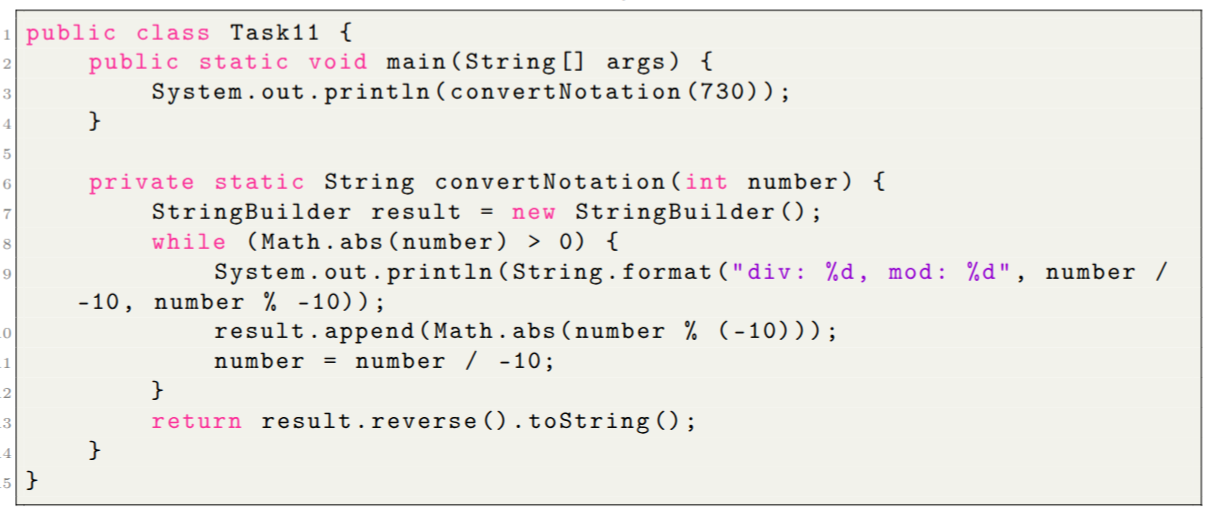
\includegraphics[width=\textwidth]{listing.png}
        % }} % ограничение области действия параметров
        \caption{Листинг кода программы на Java}
        \label{fig:java}
    \end{figure}


    \newpage

    \Section{Вывод}
        В процессе выполнения лабораторной работы по информатике я вспомнил методы перевода чисел между различными системами счисления \cite{1}, а также ознакомился и научился работать с незнакомыми мне раннее системами счисления Бергмана, фибоначчиевой и факториальной \cite{2}.
    \newpage
%<<<<<<<<<<<<<<<<<<<<<< КОД РАБОТЫ <<<<<<<<<<<<<<<<<<<<<<<<


%>>>>>>>>>>>>>>>> СПИСОК ЛИТЕРАТУРЫ >>>>>>>>>>>>>>>>>>>>>>>
    \begin{thebibliography}{}
    \bibitem{1}Орлов С. А., Цилькер Б. Я. Организация ЭВМ и систем: Учебник для вузов. 2-е изд. – СПб.: Питер, 2011. – 688 с.: ил., Приложение А «Арифметические основы вычислительных машин». URL: \url{https://bit.ly/4dzgo3u} (Дата обращения: 10.09.25) \\
    \bibitem{2}Алексеев Е.Г., Богатырев С.Д. Информатика. Мультимедийный электронный учебник. Раздел 3 «Системы счисления». URL: \url{http://inf.e-alekseev.ru/text/Schisl.html} (Дата обращения: 10.09.25)
\end{thebibliography}  % Для соответсвия гост, придется доработать. Нужен файл .bib
%<<<<<<<<<<<<<<<<<<<< СПИСОК ЛИТЕРАТУРЫ <<<<<<<<<<<<<<<<<<<

    % \Section{Список использованных источников}
    % \begin{thebibliography}{}
    %     \bibitem{1}Орлов С. А., Цилькер Б. Я. Организация ЭВМ и систем: Учебник для вузов. 2-е изд. – СПб.: Питер, 2011. – 688 с.: ил., Приложение А «Арифметические основы вычислительных машин». URL: \url{https://bit.ly/4dzgo3u} (Дата обращения: 10.09.25) \\
    %     \bibitem{2}Алексеев Е.Г., Богатырев С.Д. Информатика. Мультимедийный электронный учебник. Раздел 3 «Системы счисления». URL: \url{http://inf.e-alekseev.ru/text/Schisl.html} (Дата обращения: 10.09.25)
    % \end{thebibliography}
    \end{document}
%<<<<<<<<<<<<<<<< ,,,,,,,,,,,,,,,,,,,,,,, <<<<<<<<<<<<<<<<<
%<<<<<<<<<<<<<<<<<<< СОДЕРЖИМОЕ ОТЧЕТА <<<<<<<<<<<<<<<<<<<<